\documentclass{scrartcl}
\usepackage[T1]{fontenc}
\usepackage[utf8]{inputenc}
\usepackage[ngerman]{babel}
\usepackage{amsmath,amssymb}
\usepackage{graphicx}
\usepackage{enumerate}
\newcommand{\rbt}{Rot-Schwarz-Baum }


\begin{document}
\section*{Wissensfragen: Aufgabe 1}
\begin{enumerate}[(1)]

\item Nennen Sie zwei in der Vorlesung vorgestellte Algorithmen, die nach dem Greedy-Prinzip arbeiten. Begründen Sie kurz, warum.

\item Nennen Sie einen Vorteil und einen Nachteil von Mergesort gegenüber Quicksort.

\item Was bedeutet Stabilität bei Sortieralgorithmen? Nennen Sie eine Situation, in der man die Stabilität ausnutzen kann.

\item Bin\"are Suche hat auf jeder Datenstruktur eine bessere Laufzeit als Lineare Suche - Beweisen oder widerlegen sie diese Aussage.

\item Der zweitbeste MST ist eindeutig - Beweisen oder Widerlegen sie diese Aussage

\item Ein Algorithmus Dijkstra2 arbeitet wie Dijkstra, mit der einzigen Abwandlung, dass die Elemente in der Priorit\"atswarteschlange absteigend statt wie in Dijkstra aufsteigend sortiert sind und der Relaxierungsschritt als \newline

\textbf{if} $w_{neu}\left(e \right) > w_{alt} \left(e \right)$ \textbf{then} $w_{alt}\left( e \right) = w_{neu} \left( e \right) $ 
\newline
\newline
definiert ist.

Beweisen oder widerlegen sie die Behauptung:
Dijkstra2 findet den l\"angsten Pfad in einem Graphen ohne negative Kantengewichte. 

\end{enumerate}

\section*{Laufzeit: Aufgabe 2}
\begin{enumerate}[(1)]

\item Gegeben sei ein Datentyp, dessen Elemente bez\"uglich < bzw. > vergleichbar sind. Im folgenden betrachten wir Datenstrukturen f\"ur Elemente dieses Typs.
\begin{enumerate}[(a)]
\item Warum l\"asst sich in einem Heap das Minimum nicht in $\Theta(1)$ entfernen, so dass die entstehende Struktur immer noch ein Heap ist? \newline
Tipp: Analysieren Sie die Laufzeit des sich ergebenden Heapsorts.
\item Geben Sie eine Datenstruktur an, die die entsprechende Eigenschaft aus (a) hat.
\item Warum ist dies kein Widerspruch zur \"Uberlegung aus (a)?
\end{enumerate}

\item L\"osen Sie folgende Rekurrenzgleichungen:
\begin{enumerate}[(a)]
\item $T(n)=T(\frac{n}{2})+n$
\item $T(n)=2\cdot T(\frac{n}{2})+1$
\item $T(n)=T(\frac{n}{2})+1$
\end{enumerate}

\item Warum l\"asst sich das Mastertheorem nicht auf folgende Gleichungen anwenden?
\begin{enumerate}[(a)]
\item $T(n)=T(\frac{n}{2})+\log(n)$
\item $T(n)=n\cdot T(\frac{n}{2})+1$
\item $T(n)=T(\frac{n}{2})+n\cdot(2-\cos(n))$
\item $T(n)=T(n)+1$
\end{enumerate}

\item Seien $f,g,h,j: \mathbb{N}\to\mathbb{N}_0$ monoton wachsend. Zeigen oder widerlegen Sie:
\begin{enumerate}[(a)]
\item $f\in\Theta(g)$ und $h\in\Theta(j)\Rightarrow f\circ h \in \Theta(g\circ j)$
\item $f\in\Theta(g)$ und $h\in\Theta(j)\Rightarrow f\cdot h \in \Theta(g\cdot j)$
\item $f\in\Theta(g)$ und $h\in\omega(j)\Rightarrow f + h \in \Theta(g + j)$
\item $f\in o(g)\Rightarrow h\circ f \in o(h\circ g)$
\item $f\in O(g)\Rightarrow h\circ f \in O(h\circ g)$
\item $f\in o(g)\Rightarrow h\circ f \in O(h\circ g)$
\item $f\in O(f^2)$
\item $f\in o(f^2)$
\item $f\in \Theta(f^2)$
\end{enumerate}

\end{enumerate}

\section*{Sortieren: Aufgabe 3}
\begin{enumerate}[(1)]

\item Gegebenen sei der Sortieralgorithmus \emph{Cocktail-Sort}. Um ein Array zu sortieren, durchschreitet der Algorithmus den Array zun\"achst von vorne nach hinten und vertauscht dabei zwei benachbarte Werte, wenn sie in der falschen Reihenfolge stehen. Ist der Algorithmus am Ende des Arrays angekommen, durchschreitet er das Array jetzt in umgekehrter Reihenfolge von hinten nach vorne (also \glqq zur\"uck\grqq).
\begin{enumerate}[(a)]
\item Wenden Sie Cocktail-Sort auf folgendes Array an. Geben Sie dabei das Array nach jedem Schritt an. \\
\\
\begin{center}
\begin{tabular}{|c|c|c|c|c|c|}
\hline
4 & 2 & 1 & 3 & 7 & 3 \\
\hline
\end{tabular}
\end{center}
\text{ } \\
\item Geben Sie eine naive Implementierung von \emph{Cocktail-Sort} in Pseudocode an.
\item Geben Sie eine \emph{Familie} von Zahlenarrays an, die von Bubblesort in $O(n^2)$ sortiert werden, aber von Cocktail-Sort in $O(n)$.
\end{enumerate}

\end{enumerate}



\section*{Rot-Schwarz-Bäume: Aufgabe 4}
\begin{enumerate}[(1)]

\item Schreibe die Methode $bh(x,T)$, die f\"ur jeden Knoten $x$ seine Schwarzh\"ohe zur\"uckgibt.

\item Schreibe eine Methode $check\_b\_r\_tree(T)$, die einen \rbt als Parameter nimmt und \"uberpr\"uft, ob dieser ein g\"ultiger \rbt ist.

\item \begin{enumerate}[(a)]
\item Ein \rbt habe die H\"ohe $h$. Berechne die maximale Differenz zwischen Entfernungen von der Wurzel zu den NIL-Knoten (mit kurzer Begr\"undung).
\item Konstruiere einen solchen \rbt f\"ur $h=3$.
\end{enumerate}

\item \begin{enumerate}[(a)]
\item Gegeben sei ein \rbt der H\"ohe $h$ mit genau einem roten Knoten. Dieser habe den Abstand $d$ von der Wurzel.
Berechne f\"ur jedes $n\in \mathbb{N}$ die Anzahl $a(n)$ der NIL-Knoten, die den Abstand $n$ zur Wurzel haben.
\item Ist es m\"oglich, dass $a(h)=2^h$? Begr\"unde!
\end{enumerate}

\end{enumerate}

\section*{Datenstrukturen: Aufgabe 5}
\begin{enumerate}[(1)]

\item
\begin{enumerate}[(a)]
\item Geben sie f\"ur $n\in \{0,1,2,3,4\}$ alle M\"oglichkeiten an, die Zahlen $1,\dots,n$ in einen Min-Heap einzuordnen. Der Heap soll minimale H\"ohe haben und ein rechter Unterbaum darf nicht h\"oher sein als ein linker Unterbaum desselben Knotens.
\item Welche Heaps aus (a) haben in der Arraydarstellung keine L\"ucken?
\item Stellen Sie den folgenden Heap als Array dar. Verwenden Sie $\bot$, um L\"ucken zu kennzeichnen:\newline
{\center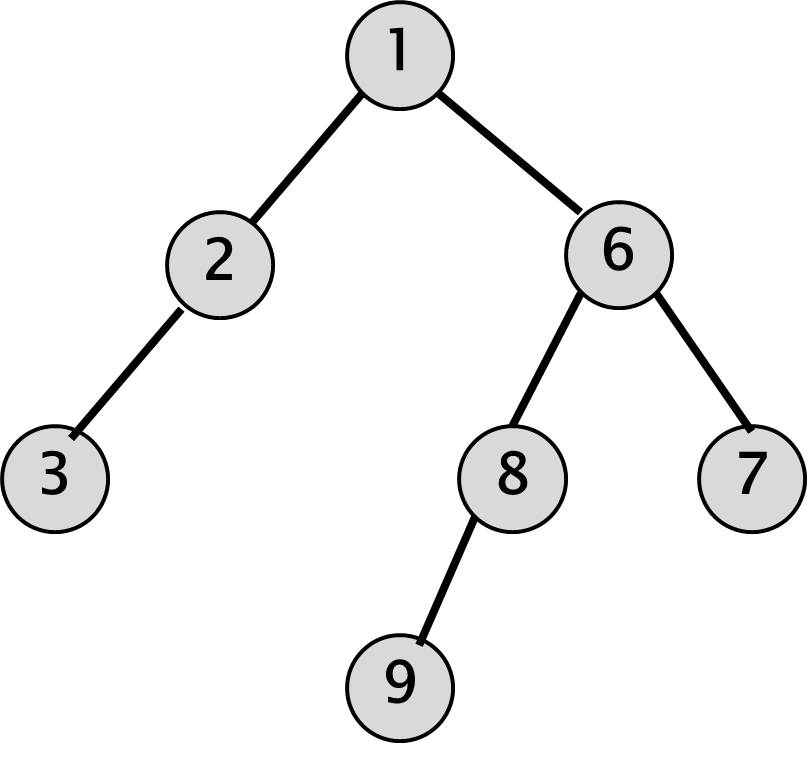
\includegraphics[scale=0.3]{images/Heap.jpg}}
\end{enumerate}

\item
Gesucht ist eine Datenstruktur, in der Einf\"ugen in konstanter Zeit ebenso m\"oglich ist wie die R\"uckgabe des minimalen Werts.
\begin{enumerate}[(a)]
\item Beschreiben Sie kurz eine m\"ogliche Datenstruktur.
\item Schreiben Sie Pseudocode f\"ur das Einf\"ugen. Es gen\"ugt, den f\"ur die sp\"atere R\"uckgabe des Minimums relevanten Teil zu betrachten.
\item Schreiben Sie Pseudocode, der das Minimum zur\"uckgibt.
\item Beschreiben Sie kurz, was beim Entfernen eines Elements passieren muss. Hat dies Auswirkung auf die Laufzeit des L\"oschens?
\end{enumerate}

\item Für die folgenden Anwendungsfälle soll jeweils eine geeignete Datenstruktur ausgewählt werden. Geben Sie jeweils eine passende Datenstruktur an und begründen Sie Ihre Wahl:
\begin{enumerate}[(a)]
\item In einer Musiksammlung sollen häufig neue Musikstücke hinzugefügt, gelöscht und gesucht werden. Über die zukünftige Größe der Sammlung kann beim Anlegen noch keine Aussage gemacht werden.
\item An einen Datenbankserver werden zu manchen Zeitpunkten so viele Anfragen geschickt, dass er sie nicht sofort bearbeiten kann. Daher soll er die Möglichkeit bekommen, die Anfragen zwischenspeichern zu können, bis er wieder genügend freie Ressourcen besitzt.
\item Ein Prozess-Scheduler in einem Betriebssystem arbeitet mit unterschiedlich hohen Prioritäten. Bei jedem Aufruf soll jeweils der Prozess mit der höchsten Priorität ausgeführt werden, wobei die Auswahlgeschwindigkeit für die Leistungsfähigkeit des Betriebssystems eine entscheidende Rolle spielt.
\end{enumerate}

\item Zeigen Sie, wie eine Warteschlange mit einer \textbf{einfach verketteten} Liste sowie zwei Zeigern \textit{K} (ältestes Element) und \textit{E} (neuestes Element) implementiert werden kann. Hierbei sollen sowohl ENQUEUE(X) als auch DEQUEUE() die Laufzeit O(1) besitzen.\\
Gehen Sie dafür folgendermaßen vor:\\
\begin{itemize}
	\item Stellen Sie mit einer Skizze dar, wie die beiden Zeiger in der Liste positioniert werden müssen.
	\item Geben Sie den Pseudocode für beide Warteschlangenoperationen an. Stellen  Sie dabei sicher, dass Ihre Implementierung auch korrekt mit einer leeren Warteschlange umgehen kann.
\end{itemize}

\end{enumerate}


\section*{Graphen: Aufgabe 6}
\begin{enumerate}[(1)]

\item Zeigen oder widerlegen Sie: Ein k\"urzester-Wege-Baum ist auch ein minimaler Spannbaum.

\item \begin{enumerate}[(a)]
\item Zeigen Sie: Dijkstra liefert bei negativen Kanten in gerichteten Graphen auch ohne negative Kreise im Allgemeinen ein falsches Ergebnis.
\item Geben Sie einen stark zusammenh\"angenden, gerichteten Graphen mit mindestens einer negativen Kante an, so dass Dijkstra f\"ur mindestens einen Startknoten ein korrektes Ergebnis liefert.
\item Warum funktioniert Dijkstra nicht auf zusammenh\"angenden, ungerichteten Graphen mit mindestens einer negativen Kante?
\end{enumerate}

\item Ein Graph G = (V,E) sei durch die folgende Adjazenzfelddarstellung gegeben:\\
\ \\
V := \begin{tabular}{|c|c|c|c|c|c|}
\hline 
1 & 3 & 4 & 6 & 9 & 11 \\ 
\hline 
\end{tabular}  \\
\ \\
E := \begin{tabular}{|c|c|c|c|c|c|c|c|c|c|c|}
\hline 
2 & 3 & 4 & 2 & 5 & 2 & 3 & 6 & 1 & 6 & 5 \\ 
\hline 
\end{tabular}\\
\begin{enumerate}[(a)]
	\item Zeichnen Sie den Graphen.
	\item Geben Sie den Graphen in Adjazenzlistendarstellung an.
	\item Welche dritte Möglichkeit zur Darstellung von Graphen wurde in der Vorlesung vorgestellt? Beschreiben Sie sie kurz und nennen Sie sowohl einen Vor- als auch einen Nachteil dieser Methode.
\end{enumerate} 

\item Wenden Sie die Algorithmen von Prim und Kruskal auf den folgenden Graphen an. Geben Sie dabei jeweils die Reihenfolge der betrachteten Kanten bzw. Knoten an.

\begin{figure}[h]
\centering
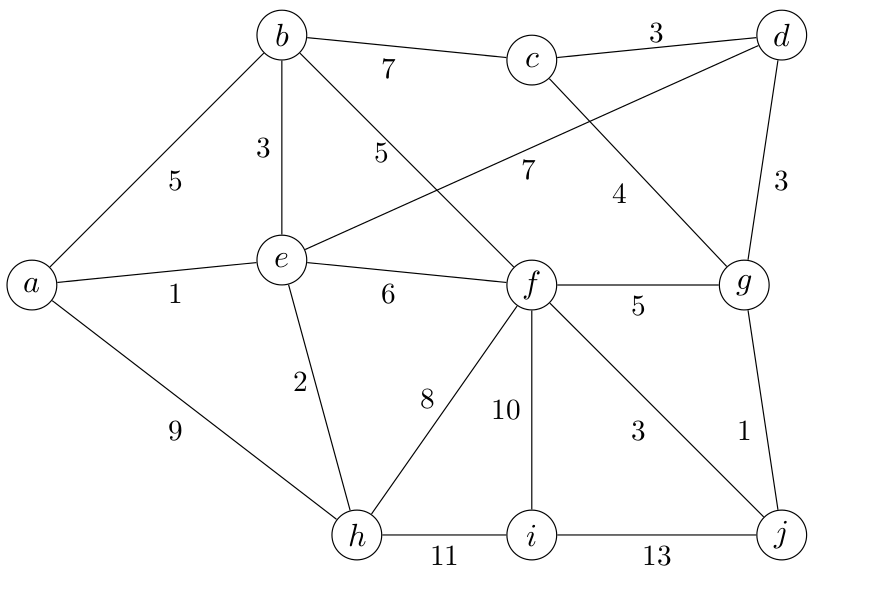
\includegraphics[width=0.66\textwidth]{mst_graph.png}
\end{figure}


\end{enumerate}

\section*{Dynamische Programmierung: Aufgabe 7}
\begin{enumerate}[(1)]

\item Was ist die grundlegende Idee hinter der Methode der dynamischen Programmierung?

\item Die Fakultätsfunktion $n!$ lässt sich folgendermaßen rekursiv definieren: \newline
$0! = 1$\newline
$n! = n\cdot(n-1)!$ 	für $n \geq 1$
\begin{enumerate}[(a)]
\item Geben Sie ein Programm in Pseudocode an, welches $n!$  mittels dynamischer Programmierung und Bottom-Up-Ansatz berechnet.
\item Das Programm soll nun so modifiziert werden, dass es nach einmaligem Berechnen von $n!$ jeden Aufruf $k!$ mit $k \leq n$ in $O(1)$ bearbeiten kann. Beschreiben Sie eine Möglichkeit dafür.
\end{enumerate}

\item Der Binomialkoeffizient $\binom{n}{k}$ kann folgendermaßen rekursiv berechnet werden:
\begin{center}
$\binom{n}{k}=\begin{cases}
0, & \text{falls } k > n;\\
1, & \text{falls } k=0 \text{ oder } n=k;\\
\binom{n-1}{k-1} + \binom{n-1}{k}, & \text{sonst.}
\end{cases}$
\end{center}
Geben Sie ein Programm in Pseudocode an, welches $\binom{n}{k}$ mittels dynamischer Programmierung und Bottom-Up-Ansatz berechnet. Hinweis: Verwenden Sie eine Matrix (d.h. ein 2-dimensionales Array), um die Lösungen der Teilprobleme zu speichern.

\end{enumerate}


\end{document}